74.  \begin{figure}[ht!]
\center{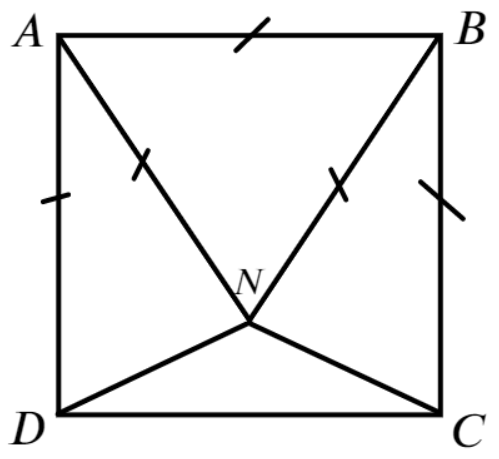
\includegraphics[scale=0.35]{g74.png}}
\end{figure}\\
Так как $ABCD$ квадрат, а треугольник $ANB$ равносторонний, имеем $AD=BC=AB=AN=BN,$ поэтому треугольники $DAN$ и $CBN$ являются равнобедренными. Углы при их вершинах равны $90^\circ-60^\circ=30^\circ,$ значит $\angle ADN=\angle BCN=(180^\circ-30^\circ):2=75^\circ.$ Таким образом, $\angle NDC=\angle NCD=90^\circ-75^\circ=15^\circ,\ \angle DNC=180^\circ-15^\circ-15^\circ=150^\circ.$\newpage
\noindent75. \begin{figure}[ht!]
\center{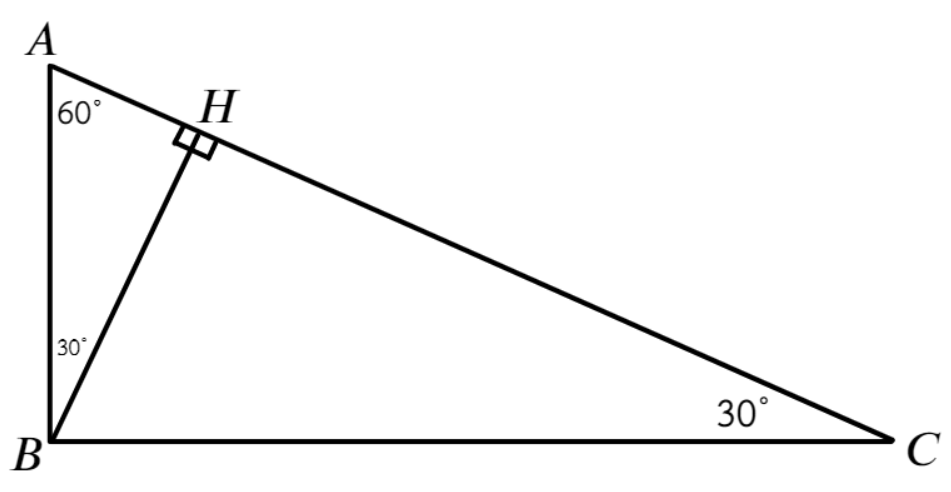
\includegraphics[scale=0.35]{g75.png}}
\end{figure}\\
Пусть $\angle C=30^\circ,$ тогда $\angle A=90^\circ-30^\circ=60^\circ,\ \angle ABH=90^\circ-60^\circ=30^\circ.$ По теореме о катете, лежащем напротив угла в $30^\circ,$ для треугольников $ABH$ и $ABC$ имеем $AB=2AH,\ AC=2AB=4AH=8,\ AH=2,\ HC=8-2=6.$\\
